\documentclass{beamer}

\mode<presentation> {
\usetheme{Madrid}
}

\usepackage{graphicx}
\usepackage{svg}
\usepackage{booktabs}
\usepackage{amsmath}
\usepackage[T1]{fontenc}
\usepackage[french]{babel}
\usepackage{url,color}
\usepackage{subfigure}
\usepackage{amsthm,amsfonts,amssymb,amscd,amsxtra, multicol}
\usepackage{comment}

\graphicspath{ {./images/} }

\title{Conception d'un SaaS pour les cours en ligne en milieu universitaire}
\author[Hans TOGNON]{Hans B. K. \textbf{TOGNON} \\ Supervisé par Ing. Miranda \textbf{GNONLONFOUN}}
\institute[IFRI]{
\textbf{I}nstitut de \textbf{F}ormation et de \textbf{R}echerche en  \textbf{I}nformatique \\
\medskip
\textbf{\color{purple}\href{mailto:contact@ifri.uac.bj}{contact@ifri.uac.bj}}
}

\begin{document}
% %%%%%%%%%%%%%%%%%%%%%%%%%%%%%%%%%%
% Title Page
% %%%%%%%%%%%%%%%%%%%%%%%%%%%%%%%%%%
\begin{frame}
  \thispagestyle{empty}
  \begin{multicols}{2}
    \begin{figure}
        \flushleft
        
\includegraphics[width=0.11\textwidth]{logoifri}
    \end{figure}
    \begin{figure}
        \flushright
        
\includegraphics[width=0.1\textwidth]{logouac}
    \end{figure}
    \end{multicols}
    \vspace{-1cm}
  \titlepage
  \end{frame}

% %%%%%%%%%%%%%%%%%%%%%%%%%%%%%%%%%%
% ToC
% %%%%%%%%%%%%%%%%%%%%%%%%%%%%%%%%%%
\begin{frame}
  \frametitle{PLAN}
  \begin{itemize}
    \item Introduction
    \item Revue de Littérature
    \item Matériels et méthodes
    \item Résultats \& Discussion
    \item Conclusion \& Perspectives
  \end{itemize}
\end{frame}

% %%%%%%%%%%%%%%%%%%%%%%%%%%%%%%%%%%
% Introduction
% %%%%%%%%%%%%%%%%%%%%%%%%%%%%%%%%%%
\begin{frame}{Introduction}
  \begin{block}{Contexte}
    Dans le but de rendre l'enseignement plus accessible, les technologies de 
    communication en temps réel sont largement exploitées. Celà induit des coûts 
    financiers non négligeables pour les divers acteurs (étudiants, enseignants, ...etc).
  \end{block}

  \begin{block}{Problématique}
    Comment promouvoir l'emploi des cours en ligne, tout en réduisant le coût financier pour les enseignants et les étudiants ?
  \end{block}
\end{frame}

\begin{frame}{Introduction}
  \begin{block}{Objectif Général}
    Concevoir \textbf{StudX}, un prototype d'application de communication en temps réel accessible en mode non connecté, pour minimiser l'utilisation des ressources.
  \end{block}
\end{frame}

\begin{frame}{Introduction}
  \begin{block}{Objectifs spécifiques}
    \begin{itemize}
      \item Organiser les entités en sections bien définies ;
      \item Définir le calendrier des cours à tenir ;
      \item Organiser des sessions d’audio-conférence pour le déroulement des cours ;
      \item Implémenter des fonctionnalités requises pour une bonne expérience utilisateur ;
      \item Minimiser certains coûts liés à l'exploitation d'une telle solution.
    \end{itemize}
  \end{block}
\end{frame}

% %%%%%%%%%%%%%%%%%%%%%%%%%%%%%%%%%%
% Revue de Littérature
% %%%%%%%%%%%%%%%%%%%%%%%%%%%%%%%%%%
\begin{frame}{Revue de Littérature : \small{Termes}}
  \begin{block}{Formation à distance}
    Forme d’enseignement ou l’enseignant et l’étudiant sont séparés dans le temps et/ou par l’espace.
    Les cours en ligne en sont la dérivée la plus exploitée, aujourd'hui.
  \end{block}
  \begin{block}{WebRTC}
    \textit{Web Real-Time Communication}. Il s'agit d'un protocole activement exploité dans la mise en oeuvre
    d'application de communication en temps réel.
  \end{block}
  \begin{block}{SaaS}
    \textit{Software as a Service}. Il s'agit d'un modèle de distribution logicielle.
  \end{block}
\end{frame}

\begin{frame}{Revue de Littérature : \small{Solutions existantes}}
  \begin{block}{Solutions}
    \begin{itemize}
      \item Google Classrooms/Google meet
      \item Zoom
      \item Moodle/BigBlueButton
    \end{itemize}
  \end{block}
  \begin{block}{Limites}
    \begin{itemize}
      \item Modèles de souscription basés sur le nombre d'utilisateurs et parfois complexes
      \item Prise en main technique requise
      \item Pas de mode hors-ligne
      \item Consommation large de données
    \end{itemize}
  \end{block}
\end{frame}
% %%%%%%%%%%%%%%%%%%%%%%%%%%%%%%%%%%
% Matériels et méthodes
% %%%%%%%%%%%%%%%%%%%%%%%%%%%%%%%%%%
\begin{frame}{Matériels et Méthodes}
  \begin{block}{Méthode d'analyse}
    \textbf{UML} est une méthode de visualisation d’architecture
    logicielle permettant de modéliser l’architecture logicielle d’un système
  \end{block}

  \begin{block}{Choix techniques}
    Trois principaux langages de programmation sont retenus:
    \begin{itemize}
      \item Rust
      \item TypeScript
      \item Python
    \end{itemize}
  \end{block}
\end{frame}

\begin{frame}{Matériels et Méthodes : \small{UML} - \footnotesize{Diagramme de cas d'utilisation}}
  \begin{figure}[H]
    \centering
    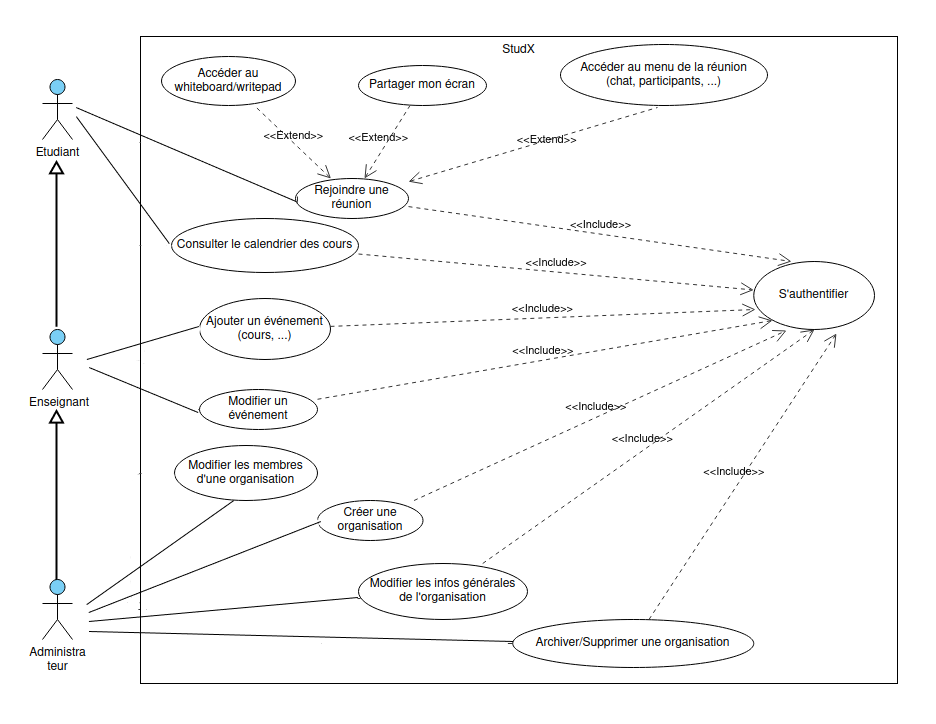
\includegraphics[width=\textwidth]{../../images/use-cases-diag.png}
    \caption{Cas d'utilisation}
\end{figure}
\end{frame}

\begin{frame}{Matériels et Méthodes : \small{UML} - \footnotesize{Diagramme de classe}}
  \begin{figure}[H]
    \centering
    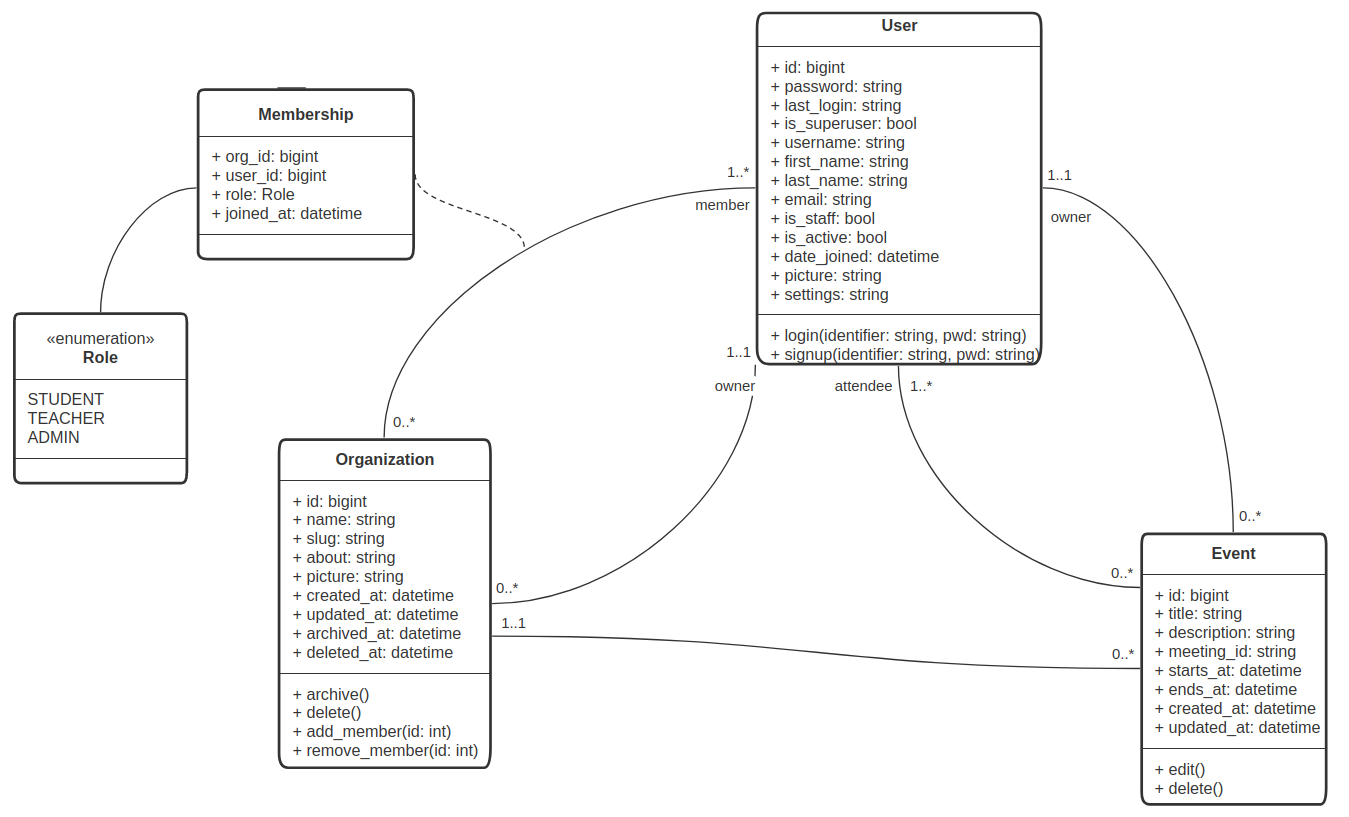
\includegraphics[width=\textwidth]{../../images/class-diag.png}
    % \caption{Diagramme de classe}
\end{figure}
\end{frame}

\begin{frame}{Matériels et Méthodes : \small{UML} - \footnotesize{Diagramme de séquence}}
  \begin{figure}[H]
    \centering
    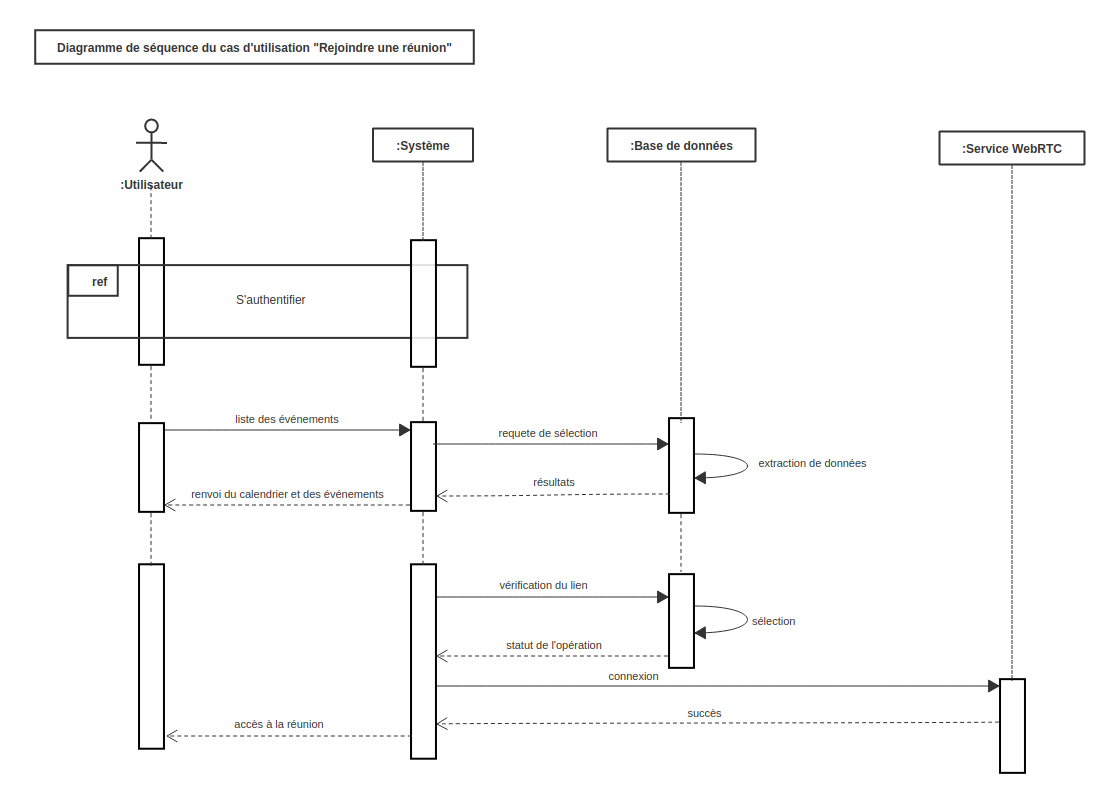
\includegraphics[width=0.9\textwidth]{../../images/join-meet-sequence-diag.png}
    % \caption{Diagramme de séquence (fonctionnalité principale)}
\end{figure}
\end{frame}

\begin{frame}{Matériels et Méthodes : \small{Implémentation du SaaS}}
  \begin{figure}[H]
    \centering
    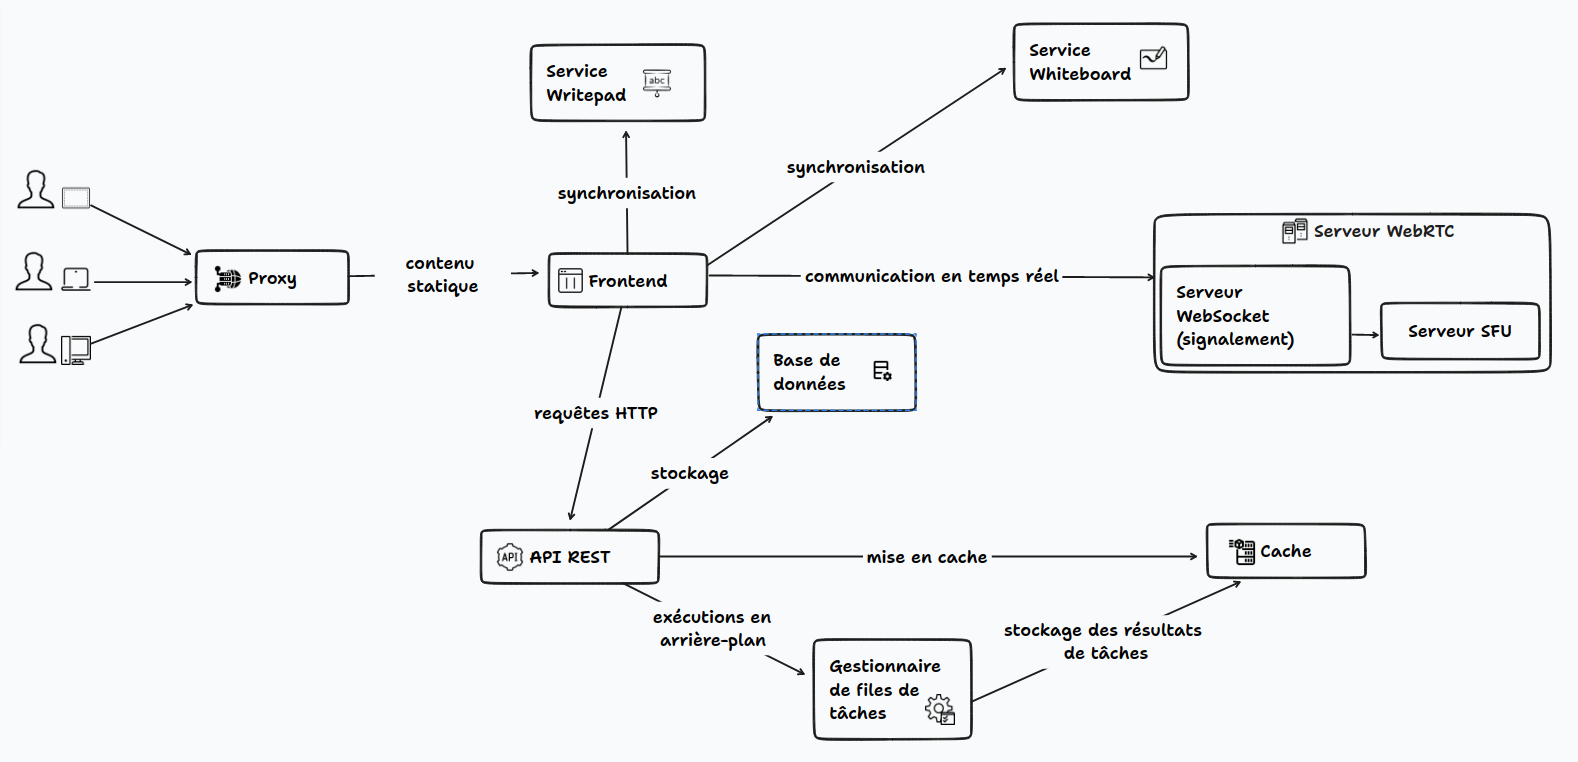
\includegraphics[width=\textwidth]{../images/studx-system-design}
    % \caption{Outils technologiques}
\end{figure}
\end{frame}

\begin{frame}{Matériels et Méthodes : \small{Technologies}}
  \begin{block}{Outils}
    \begin{itemize}
      \item Machines Physiques
      \item Machines Virtuelles
      \item Connecteur Bluetooth USB
      \item Haut-parleur Bluetooth
    \end{itemize}
  \end{block}
\end{frame}


\begin{frame}{Matériels et Méthodes : \small{Technologies}}
  \begin{figure}[H]
    \centering
    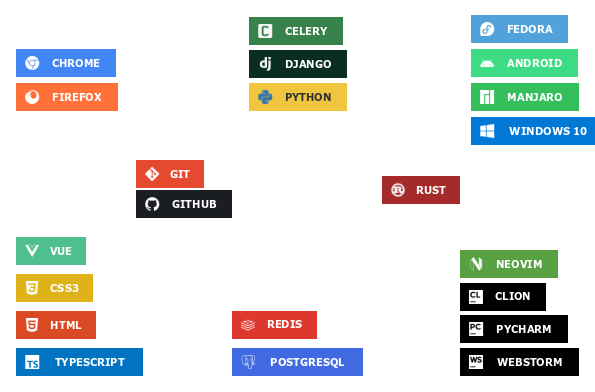
\includegraphics[width=0.9\textwidth]{tools}
    % \caption{Outils technologiques}
\end{figure}
\end{frame}

% %%%%%%%%%%%%%%%%%%%%%%%%%%%%%%%%%%
% Résultats et Discussion
% %%%%%%%%%%%%%%%%%%%%%%%%%%%%%%%%%%
\begin{frame}{Résultats \& Discussion}
  \begin{center}
    \Huge{Démonstration !}
  \end{center}
\end{frame}

\begin{frame}{Résultats \& Discussion : \small{Démonstration}}
  \begin{block}{Dispositif}
    \begin{itemize}
      \item 1 machine physique ;
      \item 1 machine virtuelle ;
      \item Chacune dispose d'une sortie audio et d'une entrée audio \textit{virtuelle} ;
      \item Elle sont toutes dans un réseau local.
    \end{itemize}
  \end{block}

  \begin{block}{Note}
    Les microphones virtuels sont alimentés par du contenu audio pour éviter de créer de l'\textit{echo}.
  \end{block}
\end{frame}

\begin{frame}{Résultats \& Discussion}
  \begin{block}{Avantages}
    \begin{itemize}
      \item Extensibilité du réseau ;
      \item Accessibilité en mode non-connecté ;
      \item Accessibilité en mode connecté ;
      \item Hébergement en mode \textit{self-hosted}.
    \end{itemize}
  \end{block}
\end{frame}

\begin{frame}{Résultats \& Discussion}
  \begin{block}{Limites}
    \begin{itemize}
      \item Persistance limitée des données ;
      \item Les sessions ne sont pas enregistrées ;
      \item L'infrastructure requise est proportionnelle au nombre d'utilisateurs.
    \end{itemize}
  \end{block}
\end{frame}

\begin{frame}{Résultats \& Discussion}
  \begin{block}{}
    La mise en place du prototype a nécéssité la mise en place et la coordination de plusieurs technologies.
    Les fonctionnalités prévues ont été implémentées. Deployée à grande échelle, l'application permet un usage en mode totalement non connecté.
  \end{block}

  \begin{block}{Code source}    
    Le code source de l'application est disponible à l'adresse suivante:
    \url{https://github.com/tobihans/studx.git}.
  \end{block}
\end{frame}

\begin{frame}{Résultats \& Discussion}
  \begin{block}{Difficultés}
    \begin{itemize}
      \item WebRTC est une technologie relativement nouvelle bien que fréquemment employée ;
      \item Il s'agit d'une technologie complexe ;
      \item Bugs liés aux navigateurs exploités (exemple: \url{https://bugs.chromium.org/p/chromium/issues/detail?id=933677}).
    \end{itemize}
  \end{block}
\end{frame}

% %%%%%%%%%%%%%%%%%%%%%%%%%%%%%%%%%%
% Conclusion et Perspectives
% %%%%%%%%%%%%%%%%%%%%%%%%%%%%%%%%%%
\begin{frame}{Conclusion \& Perspectives}
  \begin{block}{}
    Le projet développé fournit un cadre moderne de communication 
    en temps réel pour l'enseignement, avec la possibilité d'étendre ses fonctions à l'avenir;
    ceci, tout en réduisant les coûts pour les utilisateurs.
  \end{block}

  \begin{block}{Perspectives}
    \begin{itemize}
      \item Enregistrer les sessions pour un usage ultérieur ;
      \item Sauvegarder l'historique de la messagerie instantanée ;
      \item Intégrer un modèle Machine Learning pour le traitement du signal audio et sa conversion
      en langage des signes.
    \end{itemize}
  \end{block}
\end{frame}

% Thanks
\begin{frame}
  \begin{center}
  \Huge{Merci !}
  \end{center}

\end{frame}

\end{document}
